\begin{frame}[allowframebreaks]{}
    \begin{figure}
        \centering
        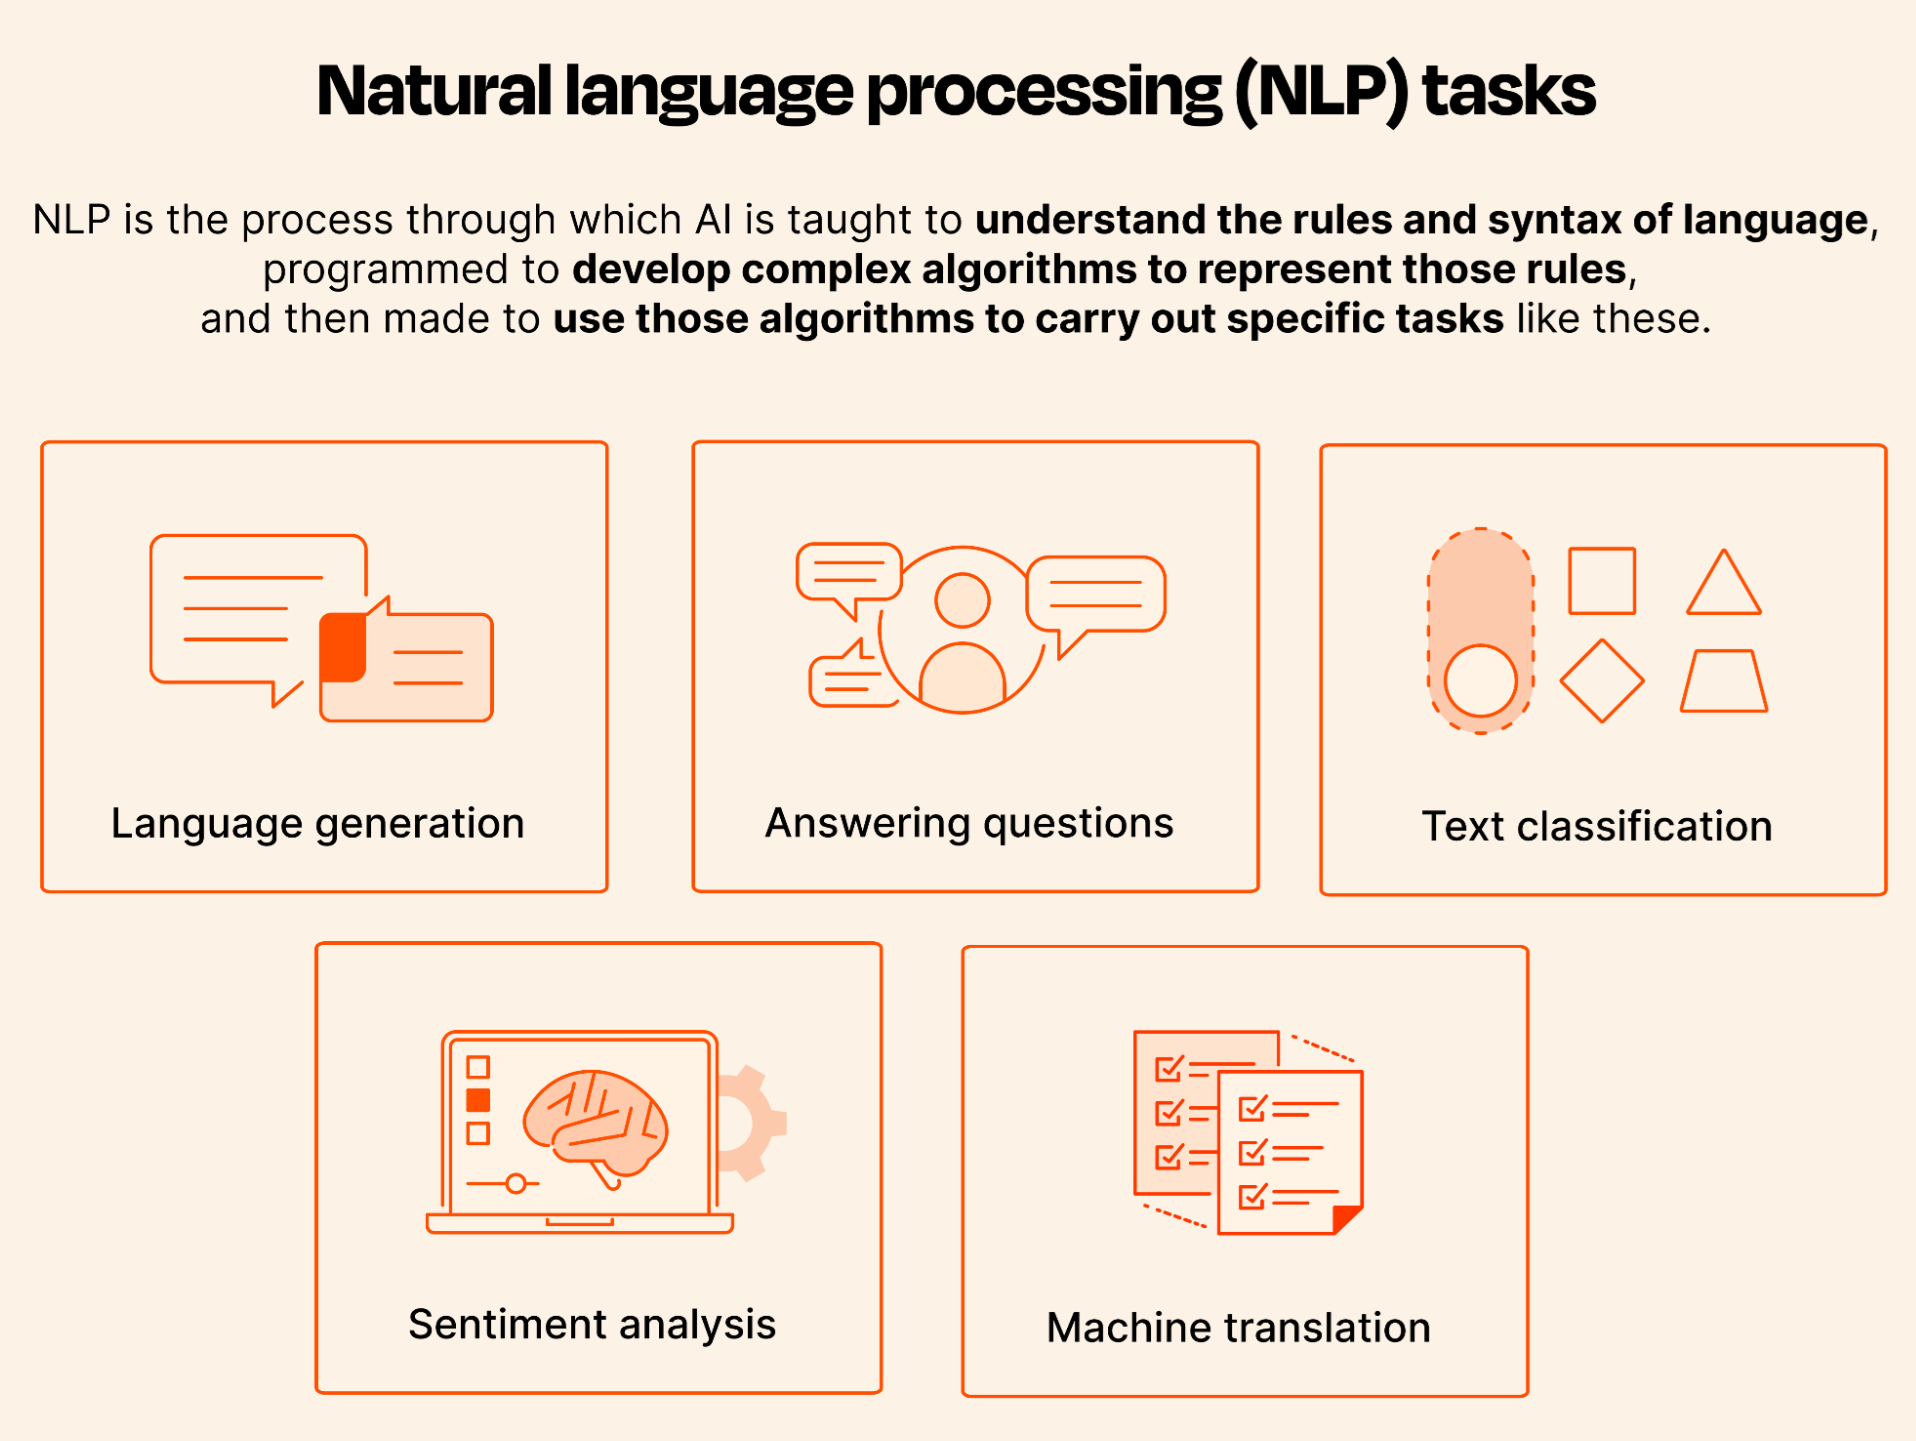
\includegraphics[height=0.9\textheight, width=\textwidth, keepaspectratio]{images/nlp/cover.png}
    \end{figure}
\end{frame}

\begin{frame}{Motivation}
    \begin{itemize}
        \item \textbf{Why NLP?}
        \begin{itemize}
            \item Humans speak different languages in many forms: text, speech, emojis!
            \item Computers don’t “understand” — they deal with 1s and 0s.
            \item NLP bridges the gap between human language and machines.
        \end{itemize}
        \item \textbf{Examples:}
        \begin{itemize}
            \item Google Translate
            \item ChatGPT
            \item Siri/Alexa
            \item Email spam filters
        \end{itemize}
        \item \textbf{Goal:} Help computers understand, interpret, and even generate human language.
    \end{itemize}
\end{frame}